\section{Einführung}

\begin{bonus}{Motivation}
    Von passiven \enquote{Informations}-Nutzung zur aktiven Nutzung.

    Neben der ursprünglichen unidirektionalen Kommunikation von Servern zu Clients, werden nun ebenfalls Daten von Clients an Server gesendet.
    Diese sind z. B. Inhalte in Foren, Podcasts, YouTube Videos etc.
    Hinzu kommen noch Webanwendungen wie Microsoft Office 365, Google Drive, Discord, draw.io etc.

    Das ursprüngliche Web bestand aus:
    \begin{itemize}
        \item Dokumenten (HTML), die eindeutig adressiert (URL) werden können und sich untereinander referenzieren.
        \item einem festen Übertragungsprotokoll: HTTP\footnote{Hypertext Transfer Protocol}
        \item Servern, die diese Dokumente Clients bereit stellen.
        \item Clients (Browsern), die diese Anfragen des Benutzenden an Server übertragen und dessen Antwort aufbereiten.
    \end{itemize}

    \begin{center}
        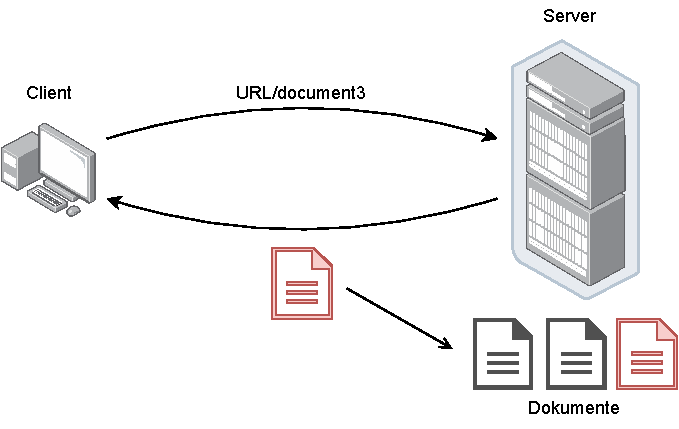
\includegraphics[width=0.5\textwidth]{includes/figures/bonus_original_web.pdf}
    \end{center}
\end{bonus}

\begin{bonus}{Klassische Client-Server-Architektur}
    Server sind langlebige Prozesse, welche auf Anfragen von Clients warten und diese abarbeiten.

    Clients stellen zu beliebigen Zeiten Anfragen und warten auf die Antwort.
\end{bonus}

\begin{defi}{Webserver}
    \emph{Webserver} sind Dienste, die Anfragen von Clients bearbeiten.

    Diese Anfragen werden von einer oder mehreren \emph{Webserver-Software} Anwendungen bearbeitet.
    Vorreiter dieser Anwendungen sind \emph{Nginx} (33.1\%) und \emph{Apache} (30.8\%).
    Ebenfalls relevant für die Klausur ist \emph{Node.js} (1.8\%).

    Die Verzeichnisstruktur ist dabei abhängig von dem Betriebssystem und Distribution:

    \begin{minipage}[t]{0.45\textwidth}
        \begin{center}
            XAMPP (Windows):
        \end{center}

        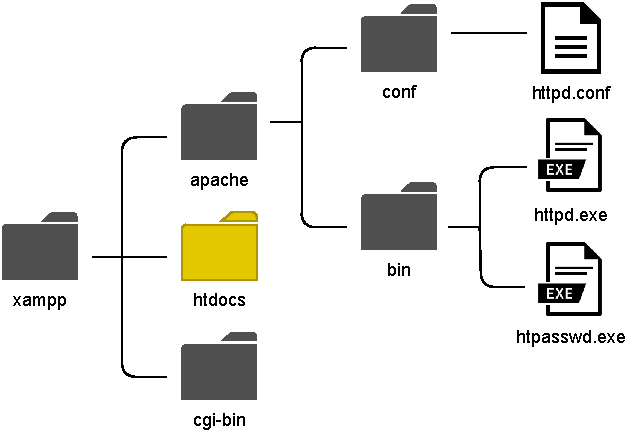
\includegraphics[width=\textwidth]{includes/figures/defi_xampp.pdf}
    \end{minipage}
    \begin{minipage}{0.1\textwidth}
        \
    \end{minipage}
    \begin{minipage}[t]{0.45\textwidth}
        \begin{center}
            Apache (Ubuntu):
        \end{center}

        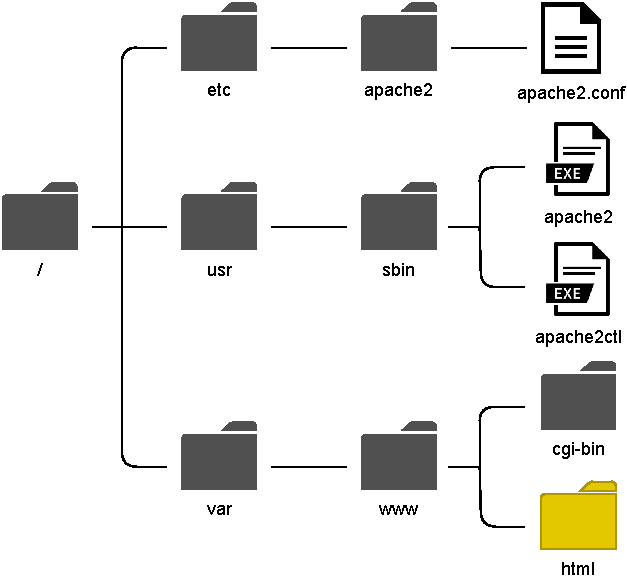
\includegraphics[width=\textwidth]{includes/figures/defi_apache.pdf}
    \end{minipage}

    \begin{center}
        \emph{Das Einstiegsverzeichnis für den Webserver ist hier gelb markiert.}
    \end{center}
\end{defi}

\begin{bonus}{XAMPP}
    \emph{XAMPP} ist ausschließlich als Entwicklungssystem geeignet!

    Viele Konfigurationen sind in Produktiveinsätzen unsicher.
    z. B. wird ein auftretender PHP Error dem Nutzenden angezeigt.
    Ebenfalls sind alle Verzeichnisinhalte zugänglich.

    Des Weiteren bietet XAMPP nur eingeschränkte (Rolling-)Update- und Clustermöglichkeiten.

    Als Produktivsystem findet man meistens Ubuntu, Debian, Red Hat oder einen Docker Container.
\end{bonus}